\documentclass{book}

% Graph - Nicht findbarer idealer gKNL impliziert wichtigen Einfluss von ISI FSI - Klappt nicht :(

% Mathematical Symbols & Physics Notation
\usepackage{amsmath}
\usepackage{amssymb}
\usepackage{physics}
\usepackage{siunitx}
\sisetup{per-mode=symbol}
\usepackage{slashed}
\usepackage{bm}

% Graphics, Diagrams & Tables
\usepackage{graphicx}
\usepackage{subcaption}
\usepackage{float}
\usepackage{tikz}
\usepackage{tikz-feynman}
\usepackage{booktabs}

% Page Layout & Head-/Footline
\usepackage[a4paper]{geometry}
\usepackage{fancyhdr}
\usepackage{lastpage}
\pagestyle{fancy}
\fancyhf{}
\fancyhead[L]{\nouppercase{\leftmark}}
\fancyhead[R]{\thepage\ of \pageref{LastPage}}

% Language & Language-specific options
\usepackage[utf8]{inputenc}
\usepackage[english]{babel}
\usepackage[mmddyyyy]{datetime}

% References & Hyperlinks
\usepackage[colorlinks=true, linkcolor=black, urlcolor=black, citecolor=black]{hyperref}
\hypersetup{linktoc=all}
\usepackage{cleveref}
%\usepackage[backend=biber,style=numeric,sorting=none]{biblatex}
%\addbibresource{references/references.bib}
\usepackage{pdfpages}

% Personalized Commands & Macros
\renewcommand{\equationautorefname}{eq.}
\numberwithin{equation}{chapter}
\numberwithin{figure}{chapter}
\renewcommand{\figurename}{figure}
\renewcommand{\theHfigure}{\thefigure}
\newcommand{\ii}{\mathrm{i}}
\newcommand{\intd}[1]{\int \frac{\dd^4 #1}{(2\pi)^4}}
\newcommand{\dbar}{\mathchar'26\mkern-11mu \dd}
\newcommand{\p}[0]{\slashed{p}}
\newcommand{\q}[0]{\slashed{q}}
\newcommand{\g}[0]{\gamma}
\newcommand{\gellmann}[0]{\frac{\lambda^a}{2}}
\newcommand{\bs}[0]{Bethe-Salpeter }
\newcommand{\SU}[0]{\text{SU(3)}}

% Titlepage Information
\title{Todo}
\author{John-Frederik Reeg}
\date{\today}


\begin{document}

\begin{titlepage}

\centering
\vspace*{0.8cm}

\LARGE
\textbf{Module Todo}

\vspace*{1.5cm}

\Huge
\textbf{Title Todo}

\vspace*{1.2cm}

\Large
Author: \\ 
\textbf{John-Frederik Reeg} \\
Student ID: 8108244

\vspace*{1.5cm}

Submission Date: Todo \\
Supervisor: Prof. Dr. Christian Fischer \\
% Second examiner: Prof. Dr. Lorenz von Smekal

\vfill

\Large \textsc{
	Justus Liebig University Giessen \\ 
	Institute for Theoretical Physics}

\vspace*{1cm}

\end{titlepage}

\tableofcontents

\chapter{Introduction} \label{ch:1}


\chapter{Theory} \label{ch:2}

\begin{align}
	A(p^2) &= Z_2 + \frac{16\pi}{3}\, Z_2^2 \int \dbar^4 q \; \frac{A(q^2)}{q^2 A^2(q^2) + B^2(q^2)} \left[ (pq) + 2 \frac{(pk)(qk)}{k^2} \right] \frac{\alpha(k^2)}{k^2} \frac{\Lambda_\textrm{PV}^2}{\Lambda_\textrm{PV}^2 + k^2} \\
	B(p^2) &= Z_4m + 16\pi \, Z_2^2 \int \dbar^4 q \; \frac{B(q^2)}{q^2 A^2(q^2) + B^2(q^2)} \frac{\alpha(k^2)}{k^2} \frac{\Lambda_\textrm{PV}^2}{\Lambda_\textrm{PV}^2 + k^2}
\end{align}

\begin{align}
	\alpha(k^2) &= \alpha_\textrm{UV}(k^2) + \alpha_\textrm{IR}(k^2) \\
	\alpha_\textrm{IR}(k^2) &= \frac{D}{\omega^6} \pi k^4 e^{-\tfrac{k^2}{\omega^2}} \\
	\alpha_\textrm{UV}(k^2) &= \frac{2\pi \gamma_m \left(1-e^{-k^2}\right)}{\ln\left[e^2-1+\left(1+\tfrac{k^2}{\Lambda_\mathrm{QCD}^2}\right)^2\right]}
\end{align}

\begin{align}
	\Xi_A(p, q) =& \int\limits_0^\pi \dd \psi \; \sin^2\psi \left[ (pq) + 2 \frac{(pk)(qk)}{k^2} \right] \frac{\alpha(k^2)}{k^2} \\
	\Xi_B(p, q) =& \int\limits_0^\pi \dd \psi \; \sin^2\psi \frac{\alpha(k^2)}{k^2} \\
	&k = p - q, \quad (pq) = |p|\.|q|\. \cos\psi
\end{align}

\begin{align}
	\begin{tikzpicture}
		\begin{feynman}
			\vertex (a1);
			\vertex[right=1.4cm of a1] (a2);
			\vertex[right=1.4cm of a2] (a3);
			\diagram* {
				(a1) -- (a2) -- (a3),
			};
			\node at (a2) [circle, fill, inner sep=1.6pt] {};
		\end{feynman}
	\end{tikzpicture}^{-1}
	\quad = \quad
	\feynmandiagram [medium, layered layout, horizontal=a to b] {
		a [particle=\(\)] -- b -- c 
	};^{-1}
	\quad - \quad
	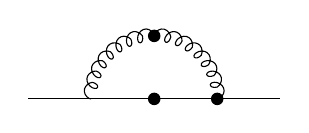
\begin{tikzpicture}
		\begin{feynman}
			\vertex (a1);
			\vertex[right=0.8cm of a1] (a2);
			\vertex[right=0.8cm of a2] (a3);
			\vertex[right=0.8cm of a3] (a4);
			\vertex[right=0.8cm of a4] (a5);
			\vertex[above=0.8cm of a3] (b1);
			\diagram* {
				(a1) -- (a2) -- (a3) -- (a4) -- (a5),
				(a4) -- [gluon, quarter right] (b1) -- [gluon, quarter right] (a2),
			};
			\node at (a3) [circle, fill, inner sep=1.6pt] {};
			\node at (a4) [circle, fill, inner sep=1.6pt] {};
			\node at (b1) [circle, fill, inner sep=1.6pt] {};
		\end{feynman}
	\end{tikzpicture}
\end{align}

\begin{figure}[H]
	\centering
	\begin{minipage}{0.9\linewidth}
		\centering
		\begin{subfigure}[t]{0.49\textwidth}
			\centering
			% \includegraphics[width=\textwidth]{images/dcs1.pdf}
			\caption{\phantom{i}}
			\label{fig:dcs1}
		\end{subfigure}\hfill
		\begin{subfigure}[t]{0.49\textwidth}
			\centering
			% \includegraphics[width=\textwidth]{images/dcs2.pdf}
			\caption{\phantom{i}}
			\label{fig:dcs2}
		\end{subfigure}
		\caption{  } 
		\label{fig:todo}
	\end{minipage}
\end{figure}


\chapter{Conclusion and Outlook} \label{ch:6}

\appendix

\chapter{Mathematical Relations}
\section{Dirac algebra} \label{ch:A}
The Dirac algebra is the algebra of the gamma matrices $\g^\mu$ used in the Dirac equation. It is defined by the anticommutation relation
\begin{align}
	\{ \g^\mu,\, \g^\nu \} = 2\,\eta^{\mu\nu} \,\mathbf 1,
\end{align}
where $\eta^{\mu\nu}$ is the defining metric of the space for which the gamma matrices are formulated, or the signature of the dot product of two four vectors.
This ensures the Lorentz covariance of the equation. The gamma matrices are represented by four $4\times4$ matrices and generate the Clifford Algebra ${\displaystyle {\text{Cl}}_{1,3}(\mathbb {C} )}$. It is also customary to define a fifth matrix, $\g^5$, which satisfies the following relations:
\begin{align}
	\{ \g^5,\, \g^\mu \} = 0\,,\hspace{1.2cm} \g^5 = (\g^5)^\dagger\,, \hspace{1.2cm} (\g^5)^2 = \mathbf 1
\end{align}
Independent of the representation, we define the Feynman-Slash operator to be:
\begin{align*}
	\p = \g_\mu p^\mu
\end{align*}

\subsection{Minkowski representation}
The metric of Minkowski space is given by the signature $(+, -, -, -)$, written as a matrix:
\begin{align}
	g_{\mu\nu} =
	\begin{pmatrix}
		1 & 0 & 0 & 0 \\
		0 & -1 & 0 & 0 \\
		0 & 0 & -1 & 0 \\
		0 & 0 & 0 & -1
	\end{pmatrix}
\end{align}
One representation of the gamma matrices that satisfies the Dirac algebra with this metric is
\begin{align}
	\g^0 = 
	\begin{pmatrix}
		1 & 0 \\
		0 & -1
	\end{pmatrix},\hspace{0.5cm}
	\g^n = 
	\begin{pmatrix}
		0 & \sigma_n \\
		-\sigma_n & 0
	\end{pmatrix},
\end{align}
where every $0$ represents an empty $2\times2$ matrix and every $1$ represents the $2\times2$ identity matrix. The $\sigma_n$ serve as placeholders for the three Pauli matrices:
\begin{align}
	\sigma_1 =
	\begin{pmatrix}
		0 & 1\\
		1 & 0
	\end{pmatrix}
	\quad
	\sigma_2 =
	\begin{pmatrix}
		0 & -\ii \\
		\ii & 0
	\end{pmatrix}
	\quad
	\sigma_3 =
	\begin{pmatrix}
		1 & 0\\
		0 & -1
	\end{pmatrix}
\end{align}
The fifth gamma matrix can now be calculated using the equation:
\begin{align}
	\g^5 = \g_5 = \ii \g^0 \g^1 \g^2 \g^3 = 
	\begin{pmatrix}
		0 & 1 \\
		1 & 0
	\end{pmatrix}
\end{align}
Furthermore we make use of the charge conjugation operator $C$, which possesses properties independent of the representation in which it is given, namely:
\begin{align}
	C^{-1} \g_\mu C = -\g_\mu^T \,,\hspace{1.2cm} C\g_5 C^{-1} = \g_5^T
\end{align}
In Minkowski space, it is represented by the matrix
\begin{align}
	C = -C^T = -C^\dagger =
	\begin{pmatrix}
		0 & \ii \sigma_2 \\
		\ii \sigma_2 & 0
	\end{pmatrix}.
\end{align}
\subsection{Euclidean representation} \label{sec:euclid}
When working in Euclidean space, it is customary to switch the indices $0$ and $4$. This also serves to differentiate clearly between four vectors in both representations. The space-like components keep the indices $1$ through $3$. Since the defining metric in Euclidean space is just the identity, the new gamma matrices need to satisfy 
\begin{align}
	\{ \g^\mu,\, \g^\nu \} &= 2\,\delta^{\mu\nu} \,\mathbf 1, \\
	\{ \g^5,\, \g^\mu \} &= 0\,.
\end{align}
They can be computed with 
\begin{align}
	\g_{n,E} &= -\ii \,\g_{n,M}, \\
	\g_{4,E} &= \g_{0,M},
\end{align}
where $n \in \{1,2,3\}$. These new representations now satisfy the anticommutation relations for this Euclidean signature. \\
Regarding $\g_5$ and $C$, both are unchanged by this new metric:
\begin{align}
	\g_{5,E} = -\g_{1,E} \, \g_{2,E} \, \g_{3,E} \, \g_{4,E} = \g_{5,M}
\end{align}\vspace*{-0.6cm}
\begin{align}
	C_E = C_M = \g_{2,E} \, \g_{4,E}
\end{align}
In this work the Euclidean metric is used primarily. Due to this, the index $E$ will be dropped and it is assumed that every gamma matrix is used in its Euclidean representation unless stated otherwise. \\
One very important note is that when working with the Euclidean metric as defined above, the invariant square of a four vector is opposite in sign to its Minkowski counterpart. To counteract this change, all four vector products in Minkowski space need to change their sign when transferred to Euclidean space:
\begin{align}
	p_E^\mu q_{\mu,E} = -p_M^\mu q_{\mu,M}
\end{align}

\section{Hyperspherical Coordinates} 
Over the course of this work it often becomes necessary to integrate over four dimensions. To facilitate this we utilize hyperspherical coordinates, with their general position vector being given by
\begin{align}
	p = |p| \begin{pmatrix} \cos\phi\sin\theta\sin\psi \\ \sin\phi\sin\theta\sin\psi \\ \cos\theta\sin\psi \\ \cos\psi \end{pmatrix}, \label{sec:hyper}
\end{align}
where $|p|$ represents the magnitude of the vector, and $\theta$, $\phi$, and $\psi$ are the angles parameterizing its direction. \\
To integrate over this coordinate system, we calculate the Jacobian and get:
\begin{align}
	\int \dd ^4p = \int\limits_0^\infty \dd p \, p^3 \int\limits_0^{2\pi}\dd \phi \int\limits_0^\pi\dd \theta \, \sin\theta \int\limits_0^\pi \dd \psi \, \sin^2\psi \label{eq:hyper}
\end{align}
Again we keep in mind the translation from Minkowski to Euclidean space, which necessitates us to bring in another factor $\ii$. 
\begin{align}
	\int \dd ^4p_M &\rightarrow \ii \int \dd ^4p_E
\end{align}
% wick
\section{Dirac Spinors in Euclidean Space} \label{ch:C}
The solutions of the free Dirac equation are called the Dirac spinors. In Euclidean space, their representations were extracted from reference 
\begin{align}
	u_1(P) &= \sqrt{\frac{E + M}{2M}}
	\begin{pmatrix}
		1 \\
		0 \\
		\frac{P_z}{E + M} \\
		\frac{P_x + iP_y}{E + M}
	\end{pmatrix}, \\
	u_2(P) &= \sqrt{\frac{E + M}{2M}}
	\begin{pmatrix}
		0 \\
		1 \\
		\frac{P_x - iP_y}{E + M} \\
		\frac{-P_z}{E + M}
	\end{pmatrix}, \\
	v_1(P) &= \sqrt{\frac{|E| + M}{2M}}
	\begin{pmatrix}
		\frac{-P_z}{|E| + M} \\
		\frac{-(P_x + iP_y)}{|E| + M} \\
		1 \\
		0
	\end{pmatrix}, \\
	v_2(P) &= \sqrt{\frac{|E| + M}{2M}}
	\begin{pmatrix}
		\frac{-(P_x - iP_y)}{|E| + M} \\
		\frac{P_z}{|E| + M} \\
		0 \\
		1
	\end{pmatrix},
\end{align}
for a given four momentum of the form $P = \left( P_x,\, P_y,\, P_z,\, \ii E \right)$. They are normalized with the conditions:
\begin{align}
	u_r^\dagger(P)\, u_{r'}(P) &= \frac{|E|}{M}\, \delta_{r,r'} \\
	u_r^\dagger(P) &= u_r^*(P)\, \gamma_4
\end{align}

\chapter{Kinematics} \label{ch:D}
This chapter seeks to visualize the kinematics of the reactions taking place. It serves to explain conventions and chosen reference frames, while also deriving the momenta used in the work above. 
\section{Breit System} \label{sec:breit}
The Breit system is a frame of reference often used to describe scattering processes. In it, we demand that the current coupling with a particle transfers only spatial momentum, so the transferred energy $Q_4$ is zero. Also known as the "brick wall frame" or "infinite momentum frame", the collision can therefore be understood as an ideal reflection on an outside particle, at least if the scattered particle does not change its mass. In the context of this work we use the Breit system to describe the coupling of a meson to a baryon, so for the calculation of the form factors
\subsection{Pion-Nucleon-Nucleon Coupling}
To calculate the kinematics of a pion-nucleon coupling in the Breit frame, we choose our coordinates so that all $x$ and $y$ momenta are 0:
\begin{align}
	Q = Q_3 \hat e_3, \quad P_{i,3} = -P_{f,3}
\end{align}
Considering momentum conservation results in the following four momenta:
\begin{align}
	Q &= \left( 0,\, 0,\, Q_3,\, 0 \right) \\
	P_i &= \left( 0,\, 0,\, -\tfrac{1}{2} Q_3,\, \ii \sqrt{M_p^2 + \tfrac{1}{4} Q_3^2} \right) \\
	P_f &= \left( 0,\, 0,\, +\tfrac{1}{2} Q_3,\, \ii \sqrt{M_p^2 + \tfrac{1}{4} Q_3^2} \right) \label{eq:kin_gpNN}
\end{align}
\subsection{Kaon-Nucleon-Lambda Coupling}
The result from above cannot simply be copied, unfortunately. In the case of nucleon-kaon absorption, the resulting lambda baryon is heavier than the incoming proton. For this to be possible without energy transfer by the kaon, the spatial momentum of the outgoing particle needs to be different in magnitude than its incoming counterpart. Again working only in $z$-direction and taking both energy and momentum conservation into account, we formulate the following four momenta, parameterized by the momentum transfer $Q$.
\begin{align}
	Q &= \left( 0,\, 0,\, Q_3,\, 0 \right) \\
	P_i &= \left( 0,\, 0,\, \frac{M_p^2 - M_\Lambda^2 - Q_3^2}{2Q_3},\, \ii \, \sqrt{M_p^2 + \left( \frac{M_p^2 - M_\Lambda^2 - Q_3^2}{2Q_3} \right)^2} \right) \\
	P_f &= \left( 0,\, 0,\, \frac{M_p^2 - M_\Lambda^2 + Q_3^2}{2Q_3},\, \ii \, \sqrt{M_\Lambda^2 + \left( \frac{M_p^2 - M_\Lambda^2 + Q_3^2}{2Q_3} \right)^2} \right) \label{eq:kin_gKNL}
\end{align}
Although the validity of this approach seems to be sufficiently correct at first, the kinematics break down for small momentum transfers. If the supplied momentum by the exchange meson does not suffice to create a lambda baryon, the calculation becomes problematic. Therefore we solve for the condition
\begin{align}
	M_\Lambda^2 \le E^2 = M_\Lambda^2 + \left( \frac{M_p^2 - M_\Lambda^2 + Q_3^2}{2Q_3} \right)^2,
\end{align}
which leaves us with a lower bound for the calculation of 
\begin{align}
	Q^2 \ge M_\Lambda^2 - M_p^2 =: \Lambda_\text{BF}^2 \approx \SI{0.4}{\giga\electronvolt\squared} \label{eq:condition}
\end{align}
Inserting a $Q^2$ below this threshold $\Lambda_\text{BF}^2$ will yield nonphysical results, a problem discussed further in.
\section{ in the Center of Mass System} \label{sec:com}
When analyzing moving objects, it is convenient to work in a resting frame of reference, the center of mass system (CM system). Its convenience stems from the property that at any given time the sum of all space-like momenta is 0:
\begin{align}
	\sum_i \bm p_i = 0
\end{align}
In order to describe the kinematics of the reaction  we will call the four momenta of all participating particles $P,\: \bar P,\: \Lambda,\: \bar\Lambda,$ and $K$. Now we can choose our coordinate system so that the space-like momentum of $\Lambda$ and $\bar\Lambda$ lays in the $x$-axis. The total energy $E_{cm}$ of each baryon as well as the magnitude of the space-like momentum of the protons can easily be calculated, since all baryons involved in this reaction are on-shell:
\begin{align}
	E_{cm} &= {\sqrt{\Lambda_x^2 + M_\Lambda^2}} \\
	|\bm p_{cm}| &= {\sqrt{E_{cm}^2 - M_p^2}}
\end{align}
With this, we can outline the kinematic situation of the reaction, where the angle $\theta$ is a new degree of freedom granted by the change in direction before/after the interaction. Without losing generality, we can restrict the reaction to the $x$-$y$-plane.
\begin{figure}[H]
	\centering
	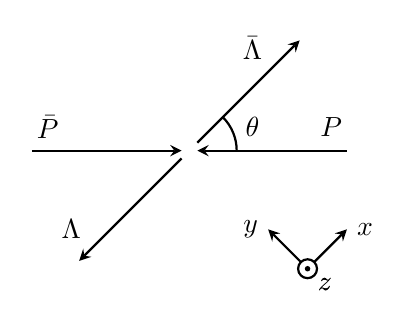
\begin{tikzpicture}[thick, >=stealth]
		\draw[->] (-2,0) -- (-0.1,0);
		\node at (-1.8, 0.3) {$\bar{P}$};
		\draw[<-] (0.1,0) -- (2,0);
		\node at (1.8, 0.3) {$P$};
		\draw[->] (-0.1,-0.1) -- (-1.4,-1.4);
		\node at (-1.5, -1) {$\Lambda$};
		\draw[->] (0.1,0.1) -- (1.4,1.4);
		\node at (0.8, 1.3) {$\bar\Lambda$};
		\draw (0.6,0) arc (0:45:0.6);
		\node at (0.8,0.3) {$\theta$};
		\draw[->] (1.58,-1.42) -- (2,-1) node[right] {$x$};
		\draw[->] (1.42,-1.42) -- (1,-1) node[left] {$y$};
		\draw (1.5,-1.5) circle (0.12) node[below right] {$z$};
		\fill (1.5,-1.5) circle (0.035) node[below right] {$z$};
	\end{tikzpicture}
	\caption{space-like momenta of the reaction}
\end{figure}
\noindent
Using this figure, we write out the four momenta of each hadron involved. Due to conservation of energy and momentum, the kaon is bound to the condition $K = \Lambda - P = \bar P - \bar\Lambda$.
\begin{align}
	P &= (-|\bm p_{cm}| \cos \theta,\: |\bm p_{cm}| \sin \theta,\: 0,\: \ii E_{cm})\\
	\bar P &= (|\bm p_{cm}| \cos \theta,\: -|\bm p_{cm}| \sin \theta,\: 0,\: \ii E_{cm})\\
	\Lambda &= (-\Lambda_x,\: 0,\: 0,\: \ii E_{cm})\\
	\bar\Lambda &= (\Lambda_x,\: 0,\: 0,\: \ii E_{cm})\\
	K &= (|\bm p_{cm}| \cos \theta - \Lambda_x,\: -|\bm p_{cm}| \sin \theta,\: 0,\: 0)
\end{align}
The center of mass energy $E_{cm}$ is shared by every hadron except the kaon, which carries no energy and is thereby off-shell and a virtual exchange particle.
\end{document}